%% Optimask Architecture
%% Created: 2017-08-02; Updated: 2017-08-02;
%% by Henghua DENG, hdeng@optixera.com

\resetdatestamp %Date Stamp--Only use when custom package datestamp.sty is used.

%\part{Optimask Layout Design} \label{PartMaskDesign}
%本部分介绍Optimask版图设计软件基本框架,具体功能实现,主要界面,命令行及编程输入等等。

%程序代码的文本引用设置
%%%%%%Matlab语言
%\lstset{language=matlab}
%\lstset{basicstyle=\scriptsize} %%size of code text: \tiny, \scriptsize, \footnotesize, \small
%%\lstset{backgroundcolor=\color{listinggray},rulecolor=\color{blue}}
%\lstset{linewidth=\textwidth}
%\lstset{commentstyle=\color{blue}\textit,stringstyle=\upshape,keywordstyle=\scriptsize,showspaces=false}
%\lstset{frame=TRBL,frameround=tttt} %TRBL=Top/Right/Bottom/Left; lower case: single line; upper case: double line;
%\lstinputlisting[label=CodeRSoft, numbers=left,firstnumber=1,stepnumber=5,breaklines=true,caption=Example Simulation File for RSoft BeamPROP 5.1]{./Figs/Code/SSC14_92.ind}
%%%%%%C语言
\lstset{language=C++}
\lstset{basicstyle=\scriptsize} %%size of code text: \tiny, \scriptsize, \footnotesize, \small
%\lstset{backgroundcolor=\color{listinggray},rulecolor=\color{blue}}
\lstset{linewidth=\textwidth}
\lstset{commentstyle=\color{blue}\textit,stringstyle=\upshape,keywordstyle=\color{magenta}\textbf,showspaces=false}
\lstset{frame=trBL,frameround=tttt} %TRBL=Top/Right/Bottom/Left; lower case: single line; upper case: double line;
%\lstinputlisting[label=CodeRSoft, numbers=left,firstnumber=1,stepnumber=5,breaklines=true,caption=Example Simulation File for RSoft BeamPROP 5.1]{./Figs/Code/SSC14_92.ind}

\chapter{Optimask Architecture 版图基本框架} \label{ChMaskArchi}
%本章主要基于刘朝洪的文档《框架概要.docx》 20170802。路径在\optixera\optimask\dev\
%======================================================================
%Heading Settings:
\markboth{Chapter~\thechapter.~Architecture}{} %\leftmark calls #1 parameter
%\markright{ } % new right header. Only used for two-side documents.

\pagestyle{fancy}
\fancyhead[RO,RE]{}
\fancyhead[LE]{\MakeUppercase{\leftmark}}
\fancyhead[LO]{\MakeUppercase{\rightmark}}
\fancyfoot[C]{\thepage}
%%\fancyfoot[L]{\today}

本章主要阐述Optimask版图软件的框架结构和软件实现。

%======================================================================
\section{总体描述} \label{SectArchRule}
%======================================================================
\subsection{架构示意图} \label{SectArchView} 
主要术语如下。架构示意图如Figure (\ref{FigLayoutArch}):
\begin{description}
	\item[版图数据] 定义版图中的基本元素、层、版图场景的结构,一个版图就是一个版图场景对象。其他任何模块都是针对版图场景数据操作。
	\item[文件读写模块] 把各种格式的版图文件读入到通用的版图数据结构,或者把通用的版图数据结构写入到指定的格式文件。
	\item[运算模块] 根据需要把版图数据中的某个元素,或者某个层,甚至整个版图数据进行运算,诸如旋转平缩放等。
	\item[视图和UI交互] 显示版图场景,绘制版图中的各种元素如直线,圆等。包括各种控制的操作。
\end{description}

\begin{figure}[htb!p] %h--here, t--top, b--bottom, p--page;
	\centering
	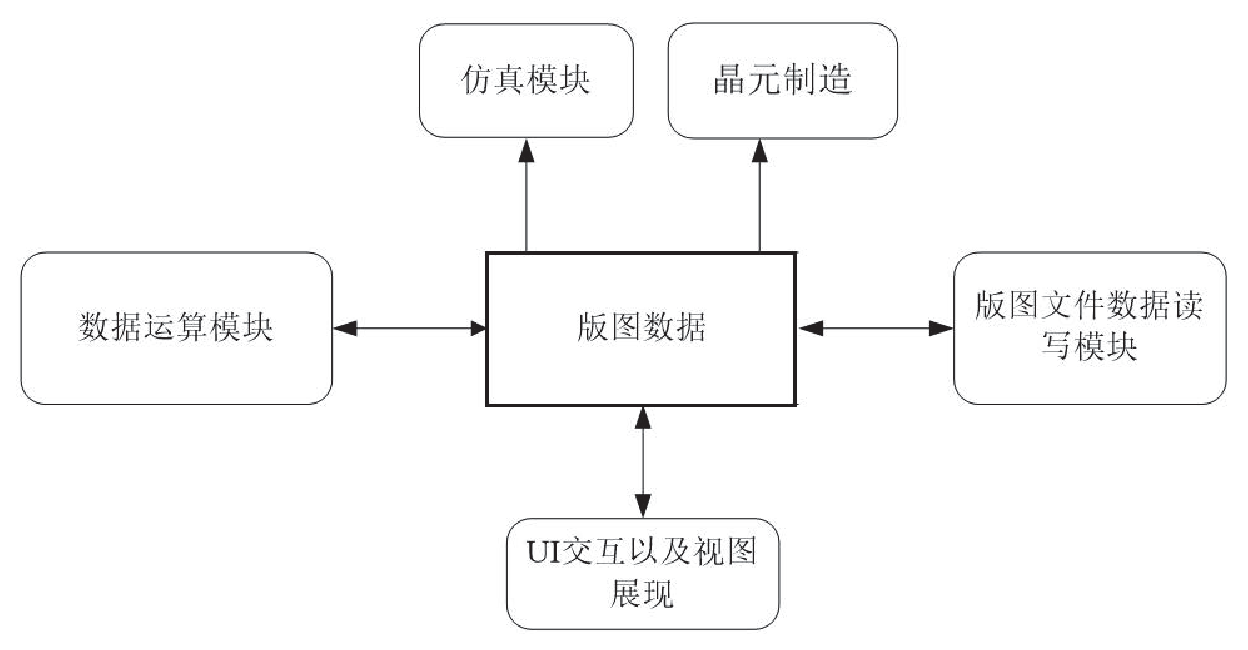
\includegraphics[width=6in]{./Layout/FigsArch/LayoutArchitect.eps}
	\caption{Optixera Software Architecture.}
	\label{FigLayoutArch}
\end{figure}

\subsection{目前存在的问题} \label{SectArchIssue} 
目前存在的问题:
\begin{enumerate}
	\item 并没有一个通用的版图数据结构,数据只是简单实用QGraphicsItem子对象来表示并保存,这样明显是没法实际操作的。以后的一些运算仿真就会比较麻烦甚至没法做。
	\item 对于版图中各种元素绘制,也是直接采用QGraphicsItem子对象来表示图元。这种方式的优点节省了代码量,很多细节不需要关心。缺点是资源耗费增大,有些特殊应用可能比较难以实现,例如也许修改会比较麻烦。我还要评估一下这样的效率和资源耗费。以及坐标转换后是否导致精度损失。
	\item 目前实现的操作好像都是针对单个图元,不能针对一组甚至全部数据。例如undo。
	\item 源代码目录结构不要随意变更
\end{enumerate}

%======================================================================
\section{基础数据结构模块} \label{SectArchData}
%======================================================================
基础数据结构模块如Figure (\ref{FigLayoutDataArch})所示。
\begin{figure}[htb!p] %h--here, t--top, b--bottom, p--page;
	\centering
	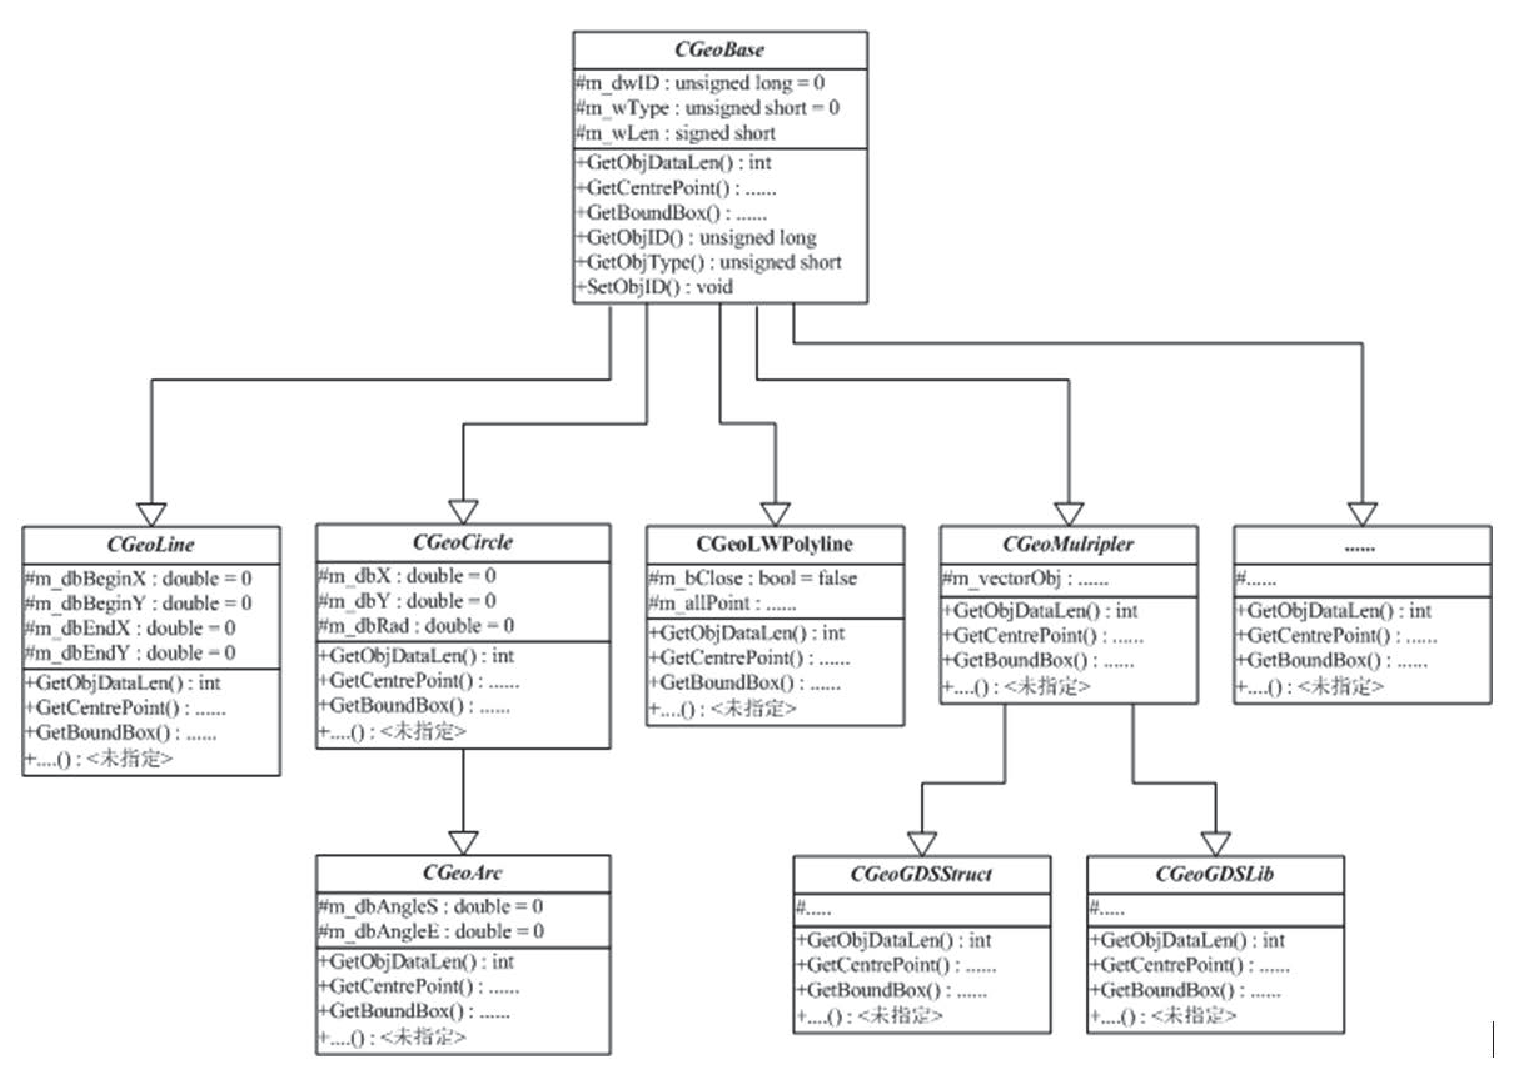
\includegraphics[width=6in]{./Layout/FigsArch/LayoutDataStructure.eps}
	\caption{Optimask Layout Data Architecture 版图数据类结构描述图样。}
	\label{FigLayoutDataArch}
\end{figure}

%======================================================================
\section{版图文件读写模块} \label{SectArchFileRW}
%======================================================================
\subsection{版图数据类结构描述图样} \label{SectArchFileStrc} 
版图文件数据读写模块的代码逻辑结构如Figure (\ref{FigLayoutDataArch})所示。
\begin{figure}[htb!p] %h--here, t--top, b--bottom, p--page;
	\centering
	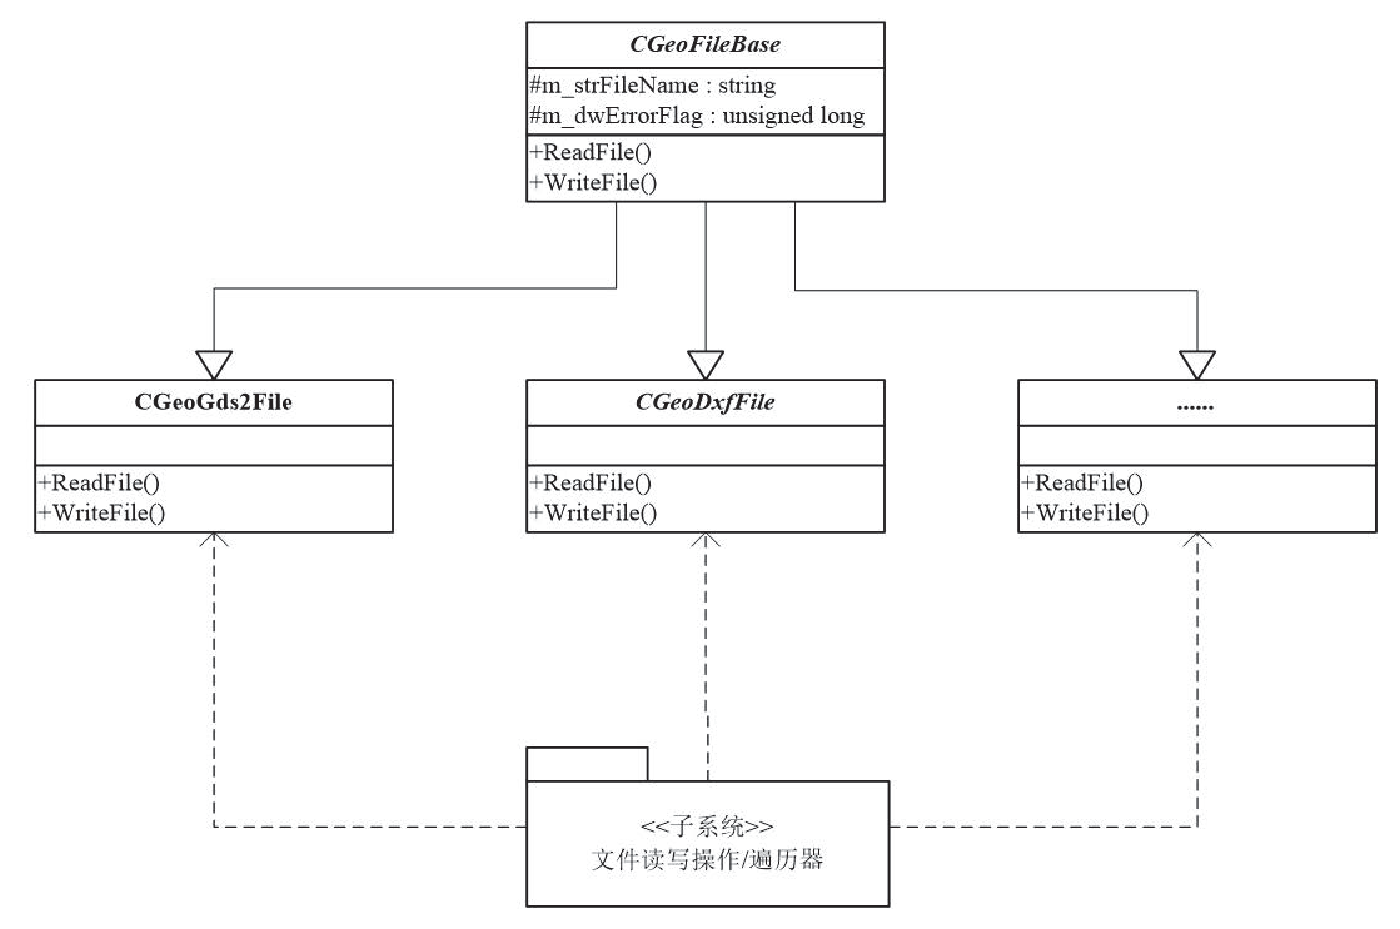
\includegraphics[width=6in]{./Layout/FigsArch/LayoutFileRWmodule.eps}
	\caption{Optimask Layout File Read/Write Module Architecture 版图文件读写模块。}
	\label{FigLayoutFileArch}
\end{figure}

\subsection{注意点描述} \label{SectArchFileNote} 
文件数据读取基类CGeoFileBase代码在GeoFile.h中,任何格式的文件实现代码必须派生与CGeoFileBase类,必须实现两个基本的虚函数ReadFile()和WriteFile(),前者是把文件数据解析成场景数据CGeoScene,后者把场景数据保存为指定格式的文件。除了两个基本的虚函数,以后可能还要添加其他的基础函数,例如GetErrorInf(),用于读取或者写入文件失败后,获取更详细的错误信息。

一个派生类至少要实现一种文件格式的读取,当然也可以同时实现几种格式的读取。对于任何格式文件的文件解析,必须实现读取函数ReadFile()用于读取指定格式的文件数据。但是根据实际情况是否特别需要,可以有选择的实现WriteFile()函数。

任何派生类都必须有缺省构造函数,因为文件读写操作/遍历器根据不同格式生成对应派生类对象时调用的是缺省构造函数。

文件读写操作/遍历器子程序包括一系列的宏定义和两个读写函数,具体列举如下:
\begin{enumerate}
	\item 全局函数$ReadDataFromFile()$和$WriteDataToFile()$
	\item 宏定义$DECLARE\_FILEFORMAT(class\_name)$声明文件格式操作链接
	\item $BEGIN_REGISTRATION(class\_name)$和$END_REGISTRATION(class\_name)$宏定义用于实现文件格式操作链接
	\item $REGISTRATION\_EXT(class\_name,ext\_name)$宏定义用于添加该类支持哪些格式解析。
\end{enumerate}

有了这些宏定义后,以后扩展或者删除其他格式解析的类代码时,只需要针对具体的格式解析类做相关的操作,其他的代码都不需要修改。因为有了这些宏的定义,$ReadDataFromFile()$和$WriteDataToFile()$函数就跟自动遍历所支持的格式类并且生成相应的类对象然后操作这些对象进行读取或者写入操作。

如$ReadDataFromFile("aaa.dxf")$。则内部根类型名找到$CGeoDXFFile$类并生成$CGeoDXFFile$对象,然偶把文件名参数以及其他的必要参数传递进入后调用$CGeoDXFFile::ReadFile()$把文件数据读取到$CGeoScene$对象中。$WriteFile()$也类似。

这些宏定义是自动遍历的基础,如果没有这些宏定义,每次增加新的格式解析类或者删除已有的格式解析类, $ReadDataFromFile()$和$WriteDataToFile()$函数代码都要相应的修改。

宏定义的使用方法:
\begin{enumerate}
	\item $DECLARE_FILEFORMAT(class\_name)$宏定义添加在每个派生的具体格式文件解析类的定义末尾,其中$class\_name$为派生类的类名。如下:
	\begin{lstlisting}[language=C]
		class CGeoDXFFile : public CGeoFileBase
		{
		……  //其他代码
		DECLARE_FILEFORMAT(CGeoDXFFile)
		};
	\end{lstlisting}
	
	\item 
	在派生类的实现文件文件中的开头添加剩下的三个宏定义,
	$BEGIN\_REGISTRATION$,$REGISTRATION\_EXT$,$END\_REGISTRATION$。
	示例如下:
	\begin{lstlisting}[language=C]
		include "GeoDxfFile.h"
		… //其他包含文件以及其他数据
		BEGIN_REGISTRATION(CGeoDXFFile)
		REGISTRATION_EXT(CGeoDXFFile, TEXT("DXF"))
		REGISTRATION_EXT(CGeoDXFFile, TEXT("DWG"))
		END_REGISTRATION(CGeoDXFFile)
	\end{lstlisting}
	
	\item
	支持一种格式,就使用$REGISTRATION_EXT(class\_name,ext\_name)$ 添加。如果支持多种格式,则每种格式都调用一次,如上的示例代码同时支持$dxf$和$dwg$格式。$class\_name$表示派生类名,$ext_name$表示支持的格式名称。
\end{enumerate}
注意:$REGISTRATION\_EXT$必须在$BEGIN\_REGISTRATION$和$END\_REGISTRATION$宏定义的中间。

%======================================================================
\section{功能清单Function CheckList} \label{SectArchFuncList}
%======================================================================
\begin{enumerate}
	\item 完善版图基础图元基础数据结构和文件数据结构定义
	\item 在Qt中实现版图基本图元自画。基本图元包括点,线,圆,圆弧,椭圆,多义线(区域)
	\item 实现基本图元的绘制数据从基础数据结构获取
	\item 在Qt中实现基本图元的选取,要注意多个图元有重叠的情况,这种情况要选取最上面的一个
	\item 实现对自画的基本图元移动缩放等处理
	\item 实现把GDS文件读入版图基础数据结构
	\item 实现版图基础数据结构数据写入到把GDS文件
	\item 实现dxf文件基本的数图元据读取
	\item 替换原先的Qt预定义图元和文档对象中的数据结构
	\item 命令行中画图调用的函数与主绘图中调用函数统一
\end{enumerate}

%======================================================================
\section{功能描述Function Description} \label{SectArchFuncDesc}
%======================================================================
根据以上的功能清单,把各个功能的开发以及一些功能实现的方案描述和工作安排。

\subsection{完善版图基础图元数据结构} \label{SectArchTaskDataStrc} 
完善版图基础图元数据结构和文件数据结构定义以及相关的数据读取功能,要求达到的最终目的如下:
\begin{enumerate}
	\item 基础数据结构完全兼容GDS2文件格式数据、大部分兼容DXF文件格式。
	\item 完善现有的GDS2文件数据读取,使之能够完整的解析出GDS2文件数据。
	\item 把读取的GDS2文件的数据转化为场景数据结构
	\item 实现把版图场景数据写入到GDS2文件中
	\item 实现把基本DXF文件数据读取到版图场景数据中
	\item 该功能估计工作量2~3周。
\end{enumerate}

\subsection{实现基本图元的绘制数据} \label{SectArchTaskDataDraw} 
实现基本图元的绘制数据从最新的版图场景数据结构中获取该功能要求绘图的数据源必须从最新定义的版图场景数据结构里面获取。以画线为例:
\begin{lstlisting}[language=C]
CGeoPt ptStart,ptEnd;
CGeoLine* temp = static_cast<CGeoLine*>(pObj);
ptStart = temp->GetFirstPt();
ptEnd = temp->GetSecondPt();
QgraphicsLineItem *item = new QgraphicsLineItem 
    (ptStart.dx, ptStart.dy, ptEnd.dx, ptEnd.dy);
item->setFlags(QGraphicsItem::ItemIsSelectable | QGraphicsItem::ItemIsMovable);
item->setPen(pen);
addItem(item);
item->setPos(0,0);
\end{lstlisting}
这个功能中的自定义在下一个功能描述中也会涉及到。这个功能由于这一步只是做一些数据源的替换实现。为了简化,可以把现有的绘制场景代码复制过来修改其中传入的参数,实现可以参考第四步。当然也可以与第四步的场景渲染结构合并一块进行,如果不合并,这个工作量比较少,估计2~3天。

\subsection{在Qt中实现版图基本图元自画} \label{SectArchTaskQtDraw} 
这个功能要求把以前在Qt中通过QGraphicsItem类的子类对象画基本图元全部改成自画,例如上一步描述的就是通过QgraphicsLineItem实现画线,经过这一步后不再使用QGraphicsItem类的子类对象实现,也不需要通过addItem(item)之类的代码把该图元添加到场景中。可以减少实现数据渲染依赖具体UI对象。

还是以上面的画线为例,修改后画图的示例代码如下:
\begin{lstlisting}[language=C]
CGeoPt ptStart,ptEnd;
CGeoLine* temp = static_cast<CGeoLine*>(pObj);
ptStart = temp->GetFirstPt();
ptEnd = temp->GetSecondPt();
QpointF tmpStart(ptStart.dx, ptStart.dy);
QpointF tmpEnd(ptEnd.dx, ptEnd.dy)

QPainter painter(this->viewport());
QPen pen(Qt::black);    
painter.setPen(pen);
painter.setBrush(Qt::black);
painter.drawLine(tmpStart, tmpEnd);
\end{lstlisting}
注意:以上代码只是一个简单的演示代码。对于实际上的场景画图,画图时不要直接画到显存上,而是要先画到位图上,然后把位图复制给显存。这些绘制可以在paintEvent事件里面画图,也可以独立,根据实际情况来。

为了方便场景数据的绘制,定义了一个场景渲染接口类CSceneRender用于封装与UI绘制无关的绘制操作,在其子类里面实现与具体的UI接口关联绘制,接口定义在SceneRender.h文件中。该接口类定义了一些基础图元绘制函数接口,由子类实现绘制。

接口定义如下,以后也许会增加或者修改接口定义
\begin{lstlisting}[language=C]
virtual void DrawScene();
virtual void DrawPrimitive(CGeoLine* pData)=0;
virtual void DrawPrimitive(CGeoCircle* pData)=0;
virtual void DrawPrimitive(CGeoArc* pData)=0;
virtual void DrawPrimitive(CGeoLWPolyline* pData)=0;
virtual void DrawPrimitive(CGeoEllipse* pData)=0;
virtual void DrawPrimitive(CGeoText* pData)=0;
virtual void DrawPrimitive(CGeoMulripler* pData)=0;
\end{lstlisting}

在上面的定义中,DrawScene()函数接口用于绘制整个场景,它的实现是遍历整个场景所有图层中的所有图元(如果某个图元有子图元,则迭代遍历,直达基本图元的叶节点),然后分别画出基本图元。
DrawPrimitive()函数分别对应着不同的基本图元实现不同的绘制方法。例如$DrawPrimitive(CGeoLine* pData)$函数的实现绘制直线,可能是如下的情况:
\begin{lstlisting}[language=C]
DrawPrimitive(CGeoLine* pData)
{
	CGeoPt ptStart,ptEnd;
	ptStart = pData ->GetFirstPt();
	ptEnd = pData ->GetSecondPt();
	如果没有实现自定义绘制,则应该是如下的代码
	QgraphicsLineItem *item = new QgraphicsLineItem
	    (ptStart.dx, ptStart.dy, ptEnd.dx, ptEnd.dy);
	item->setFlags(QGraphicsItem::ItemIsSelectable 
	    | QGraphicsItem::ItemIsMovable);
	item->setPen(pen);
	addItem(item);
	//如果采用的自定义绘图,则是类似如下的代码
	//(仅仅是示例用来表明方案,实现上根据实际情况可能采用效率更高的绘制)
	QpointF tmpStart(ptStart.dx, ptStart.dy);
	QpointF tmpEnd(ptEnd.dx, ptEnd.dy)
	QPainter painter(this->viewport());
	QPen pen(Qt::black);    
	painter.setPen(pen);
	painter.setBrush(Qt::black);
	painter.drawLine(tmpStart, tmpEnd);
}
\end{lstlisting}

场景接口类必须与具体的UI操作结合来实现绘图,绘图操作与场景渲染接口类CsceneRender结合的代码如下:
以Qt的视图绘制类为例:

\begin{lstlisting}[language=C]
class CView:public QgraphicsView, public CSceneRender
{
	Q_OBJECT
	
	….
	virtual void DrawScene();
	virtual void DrawPrimitive(CGeoLine* pData);
	virtual void DrawPrimitive(CGeoCircle* pData);
	virtual void DrawPrimitive(CGeoArc* pData);
	virtual void DrawPrimitive(CGeoLWPolyline* pData);
	virtual void DrawPrimitive(CGeoEllipse* pData);
	virtual void DrawPrimitive(CGeoText* pData);
	virtual void DrawPrimitive(CGeoMulripler* pData);
}
\end{lstlisting}

该场景类也定义了一些基本的场景图元添加删除更新操作,方便命令行功能模块调用这些接口函数实现场景相关的操作诸如添加直线等。如
AddLine()

DelObject()

命令行功能如果接收到输入添加直线的命令,解析后直接调用AddLine(),该函数自动把新增的直线添加到当前场景数据中,如果同时需要把添加的直线在视图上显示出来,则调用DrawPrimitive()函数即可。

场景渲染结构示意图如下:

\subsection{在Qt中实现自画基本图元的选取} \label{SectArchTaskQtPick} 
选取基本图元的功能是基于自定义画图,如果采取Qt的预定义绘图,则内置了选取移动等功能,选取功能不需要再次实现。

进行图元选取之前,先必须建立基于坐标位置的图元索引,建立图元索引的方案描述如下:
\begin{enumerate}
	\item 把整个场景分成n*m个栅格区域,每个栅格的编号都是根据实际坐标范围来映射,每个编号本身的含义就对应着一定的栅格区域范围。每个栅格的大小固定的。
	\item 计算栅格编号的方法:先计算出图形区域的最小坐标点$(Xmin,Ymin)$和最大坐标点$(Xmax,Ymax)$。最小坐标点向下取整,最大坐标点向上取整。为了冗余,也可以在最小坐标点再向下偏移几个单位,最大坐标点再向上偏移几个单位。然后计算出栅格的区域范围,其中宽度数据$width=(Xmax- Xmin)/n$,高度数据为$height=(Ymax- Ymin)/m$。计算出来的宽度和高度向上取整。对于任意坐标$(X,Y)$,则$X$方向的编号为$NOx =  (X- Xmin)/width$, $Y$方向的编号为$NOy =  (Y- Ymin)/ height$。两者编号都取整。实际编号就是两者编号的组合,如$NO = (NOx<<16)+ NOy$。(设定编号为32为无符号整形)。
	\item 如果图元位于栅格里面、与栅格相交、包含栅格。则这个图元就属于这个栅格。因此一个图元可能对应着多个栅格。建立一个编号与图元的多重映射,关键字为栅格编号,值为图元列表。
	\item 当图元发生平移或者选择时,需要更新该图元所在的栅格信息。
\end{enumerate}

选取的功能描述如下;
\begin{enumerate}
	\item 把选取的屏幕坐标转化为图形坐标
	\item 根据图形坐标计算该坐标所在的栅格ID
	\item 根据栅格ID找出位于该栅格的所有图元,然后继续下一步找出满足条件的图元。
	\item 把这个栅格内的所有图元的区域与选取的坐标点进行比较,如果坐标点位于区域内或者区域边界,则满足要求。如果有多个图元满足要求,则选取的原则为:就小不就大,当前层优先。意思如果多个图元都包含选取点时,则选取区域最小的那个,如果区域相同的有多个,则选取当前层的那个。另外如果当前层也有区域相同的多个(正常情况下这应该是错误,因为这是重复图元)则选列表中的第一个。
	\item 选定了基本图元,把图元的边界突出显示
\end{enumerate}

\subsection{对自画图元的平移旋转等基本操作} \label{SectArchTaskDrawAltr} 
平移旋转操作本身不是难事,现在主要说明在鼠标操作的情况:
\begin{enumerate}
	\item 选定需要操作的图元
	\item 捕获鼠标的点击与移动事件,计算出图元要平移或者旋转的屏幕距离
	\item 根据平移或者旋转操作把计算出来的屏幕距离转换成实际的平移距离或者选择的角位移
	\item 调用平移或者旋转函数
	\item 要求刷新显示
\end{enumerate}
如果是命令行,则只有后面的4,5两步。
目前需要把针对图元旋转平移的功能封装起来。

\subsection{彻底替换以前的采用Qt预定义图元操作以及文档中的场景数据} \label{SectArchTaskReplaceQt} 
彻底替换以前的采用Qt预定义图元操作以及文档中的场景数据。


%%\pagestyle{empty}
%%\cleardoublepage
%%to generates one blank page for the next chapter to be on an odd page
